\section[Section]{Rebase}

{
% Fit multiple things on a slide closer together
\setlength\partopsep{-2\topsep}

\begin{frame}
    \frametitle{Rebase}
    \centering
    With great power comes great responsibility
\end{frame}
\note[itemize]{
    \item Swiss-army-knife of rewriting history
    \item The ability to edit or rewrite history sets Git apart from other
          version control systems
}

{
\setbeamertemplate{background}{}
\setbeamertemplate{background}{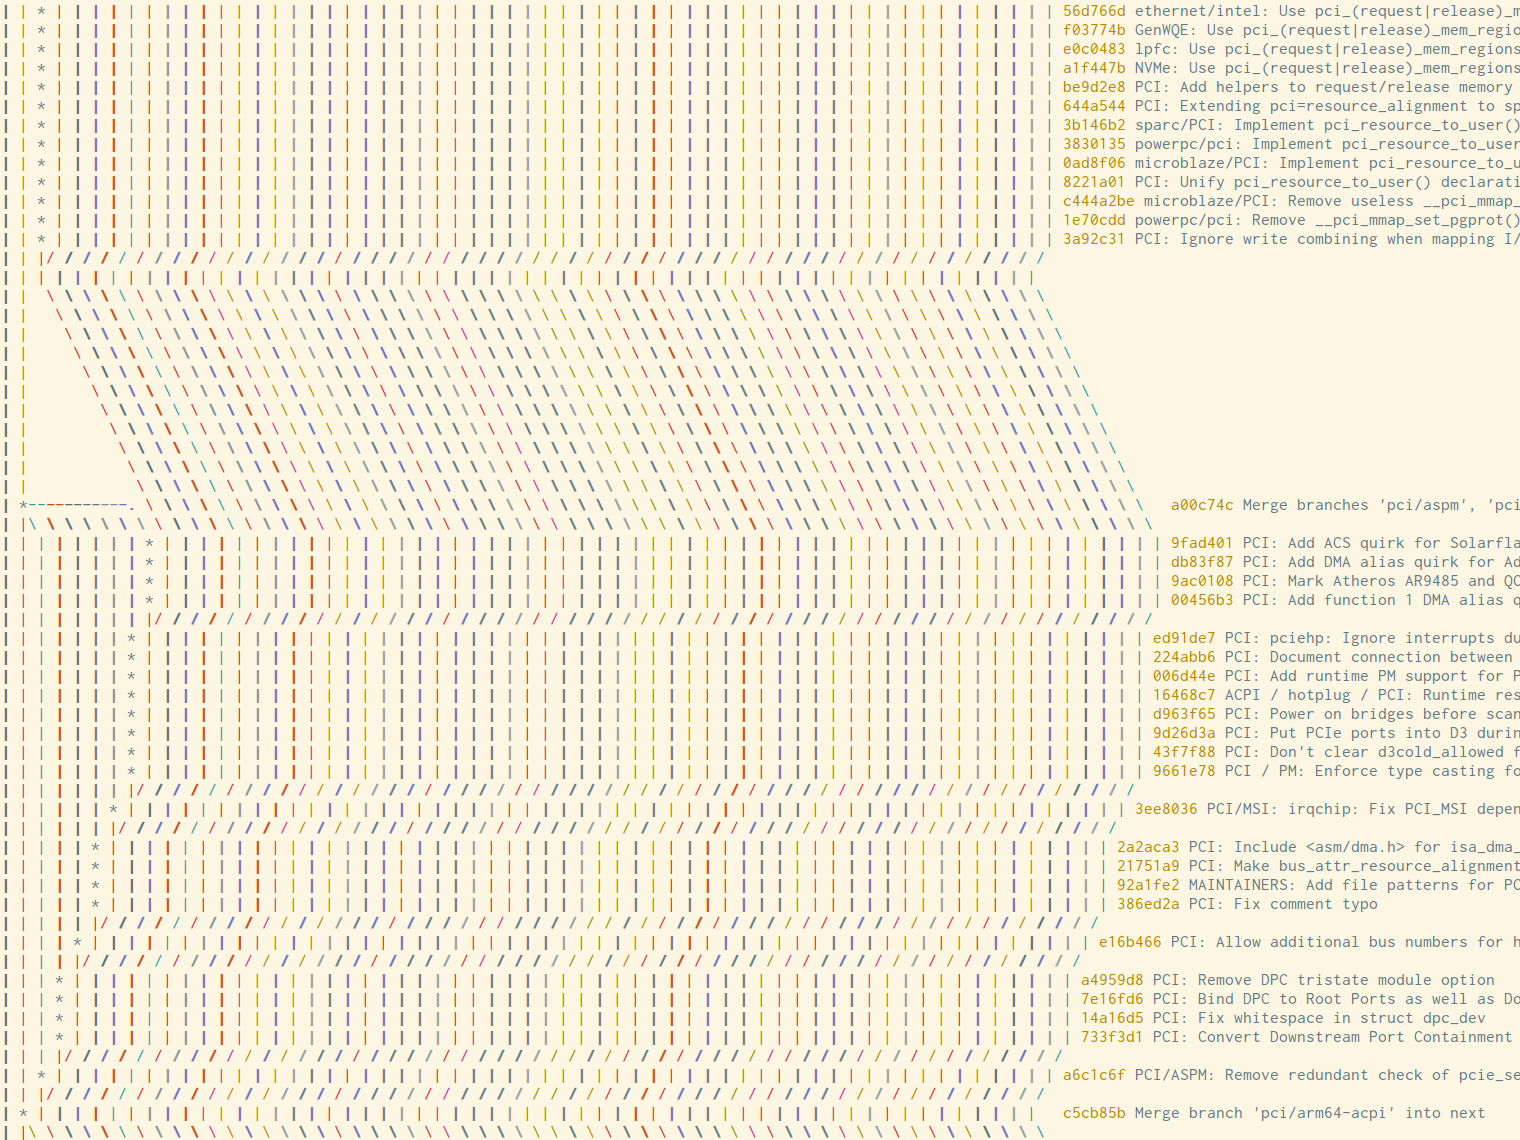
\includegraphics[width=\paperwidth]{images/linux-branches.png}}
\begin{frame}[plain]
\end{frame}
\note[itemize]{
    \item Long running branches can be confusing
    \item This is from the linux kernel
}
}

\begin{frame}
    \frametitle{Developing in Parallel or Taking Turns}
    \begin{figure}
        \begin{subfigure}[b]{\textwidth}
            \centering
            \begin{tikzpicture}
                \gitDAG[grow right sep=2em]{
                    A -- {{B, C -- D} -- H, E -- F -- G} -- I
                };
            \end{tikzpicture}
            \subcaption{Multiple Concurrent Branches}
        \end{subfigure}
        \begin{subfigure}[b]{\textwidth}
            \centering
            \begin{tikzpicture}
                \gitDAG[grow right sep=2em]{
                    A -- B -- C -- D -- E -- F -- G
                };
            \end{tikzpicture}
            \subcaption{Linear History}
        \end{subfigure}
        \caption{Two Ways to Tell a Story}
    \end{figure}
\end{frame}
\note[itemize]{
    \item What if we could use our version control tool to pretend that we took
          turns even when we develop in parallel
    \item Edit the top history to look like the bottom
    \item \alert{Question}: Is this even a good idea?
    \item The first use of \texttt{git rebase} we will look at will do this
}

\begin{frame}
    \frametitle{Rebase}
    \begin{figure}
        \centering
        \begin{tikzpicture}
            \gitDAG[grow right sep=2em]{
                A -- {{B, C -- D} -- {[nodes=unreachable] H},
                E -- F -- G} -- {[nodes=unreachable] I}
            };
            \gitbranch{master}{above=of B}{B}
            \gitHEAD{above=of master}{master}
            \gitbranch{foo}{right=of D}{D}
            \gitbranch{bar}{right=of G}{G}
        \end{tikzpicture}
        \caption{Two Branches to Rebase}
    \end{figure}
\end{frame}
\note[itemize]{
    \item Instead of creating the merge commits H and I we'll rebase foo and
          bar onto master in order to create a linear history
}

\begin{frame}[fragile]
    \frametitle{Rebase}
    \begin{figure}
        \centering
        \begin{tikzpicture}
            \gitDAG[grow right sep=2em]{
                A -- {{B, C -- D},
                E -- F -- G}
            };
            \gitbranch{master}{above=of B}{B}
            \oldgitHEAD{above=of master}{master}
            \gitbranch{foo}{right=of D}{D}
            \gitHEAD{right=of foo}{foo}
            \gitbranch{bar}{right=of G}{G}
        \end{tikzpicture}
        \caption{Checkout foo}
    \end{figure}
    \begin{minted}[bgcolor=solarized-base2!50,frame=single,framesep=3pt]{console}
$ git checkout foo
    \end{minted}
\end{frame}
\note[itemize]{
    \item First, we'll rebase foo onto master
    \item We must checkout foo first
    \item Remember Git will not touch branches you don't have checked out
    \item We want to take the branch foo, containing commits C and D, and
          reaply them after commit B
}

\begin{frame}[fragile]
    \frametitle{Rebase}
    \begin{figure}
        \centering
        \begin{tikzpicture}
            \gitDAG[grow right sep=2em]{
                A -- {{B -- C' -- D', {[nodes=unreachable] C -- D}},
                E -- F -- G}
            };
            \gitbranch{master}{above=of B}{B}
            \oldgitbranch{foo}{right=of D}{D}
            \oldgitHEAD{right=of foo}{foo}
            \gitbranch{foo}{above=of D'}{D'}
            \gitHEAD{above=of foo}{foo}
            \gitbranch{bar}{right=of G}{G}
        \end{tikzpicture}
        \caption{Rebase foo onto master}
    \end{figure}
    \begin{minted}[bgcolor=solarized-base2!50,frame=single,framesep=3pt]{console}
$ git rebase master
    \end{minted}
\end{frame}
\note[itemize]{
    \item ... to do that, we use the command \texttt{git rebase master}
    \item Commits C' and D' have the
    \begin{itemize}
        \item same deltas as C and D,
        \item same commit message,
        \item same author,
    \end{itemize}
    \item but different sha1sum because they have
    \begin{itemize}
        \item different parents,
        \item and different trees (different snapshots);
        \item because the snapshots also contain the changes in B
    \end{itemize}
    \item Rebase works by
    \begin{itemize}
        \item first finding a common ancestor (A)
        \item making patches for each commit in the source branch
        \item and reapplying them on the destination branch
    \end{itemize}
}

\begin{frame}[fragile]
    \frametitle{Rebase}
    \begin{figure}
        \centering
        \begin{tikzpicture}
            \gitDAG[grow right sep=2em]{
                A -- {{B -- C' -- D', {[nodes=placeholder] C -- D}},
                E -- F -- G}
            };
            \gitbranch{master}{above=of B}{B}
            \gitbranch{foo}{above=of D'}{D'}
            \oldgitHEAD{above=of foo}{foo}
            \gitbranch{bar}{right=of G}{G}
            \gitHEAD{above=of bar}{bar}
        \end{tikzpicture}
        \caption{Checkout bar}
    \end{figure}
    \begin{minted}[bgcolor=solarized-base2!50,frame=single,framesep=3pt]{console}
$ git checkout bar
    \end{minted}
\end{frame}
\note[itemize]{
    \item Repeat the process for branch bar
}

\begin{frame}[fragile]
    \frametitle{Rebase}
    \begin{figure}
        \centering
        \begin{tikzpicture}
            \gitDAG[grow right sep=2em]{
                A -- {{B -- C' -- D' -- E' -- F' -- G',
                {[nodes=placeholder] C -- D}},
                {[nodes=unreachable] E -- F -- G}}
            };
            \gitbranch{master}{above=of B}{B}
            \gitbranch{foo}{above=of D'}{D'}
            \oldgitbranch{bar}{right=of G}{G}
            \oldgitHEAD{above=of bar}{bar}
            \gitbranch{bar}{above=of G'}{G'}
            \gitHEAD{above=of bar}{bar}
        \end{tikzpicture}
        \caption{Rebase bar Onto foo}
    \end{figure}
    \begin{minted}[bgcolor=solarized-base2!50,frame=single,framesep=3pt]{console}
$ git rebase foo
    \end{minted}
\end{frame}
\note[itemize]{
    \item Reapply E, F, and G after D'
}

\begin{frame}[fragile]
    \frametitle{Rebase}
    \begin{figure}
        \centering
        \begin{tikzpicture}
            \gitDAG[grow right sep=2em]{
                A -- B -- C' -- D' -- E' -- F' -- G'
            };
            \gitbranch{master}{above=of B}{B}
            \gitHEAD{above=of master}{master}
            \gitbranch{foo}{above=of D'}{D'}
            \gitbranch{bar}{above=of G'}{G'}
            \oldgitHEAD{above=of bar}{bar}
        \end{tikzpicture}
        \caption{Update master}
    \end{figure}
    \begin{minted}[bgcolor=solarized-base2!50,frame=single,framesep=3pt]{console}
$ git checkout master
    \end{minted}
\end{frame}
\note[itemize]{
    \item Now that we have the version of history that we want, let's update
          master
    \item First checkout master
}

\begin{frame}[fragile]
    \frametitle{Rebase}
    \begin{figure}
        \centering
        \begin{tikzpicture}
            \gitDAG[grow right sep=2em]{
                A -- B -- C' -- D' -- E' -- F' -- G'
            };
            \oldgitbranch{master}{above=of B}{B}
            \oldgitHEAD{above=of master}{master}
            \gitbranch{foo}{above=of D'}{D'}
            \gitbranch{bar}{above left=of G'}{G'}
            \gitbranch{master}{above=of G'}{G'}
            \gitHEAD{above=of master}{master}
        \end{tikzpicture}
        \caption{Merge Changes Into master}
    \end{figure}
    \begin{minted}[bgcolor=solarized-base2!50,frame=single,framesep=3pt]{console}
$ git merge bar
    \end{minted}
\end{frame}
\note[itemize]{
    \item Merge bar into master
    \item \alert{Question}: What kind of merge is this? Fast-forward merge
}

\begin{frame}[fragile]
    \frametitle{Rebase}
    \begin{figure}
        \centering
        \begin{tikzpicture}
            \gitDAG[grow right sep=2em]{
                A -- B -- C' -- D' -- E' -- F' -- G'
            };
            \oldgitbranch{foo}{above=of D'}{D'}
            \oldgitbranch{bar}{above left=of G'}{G'}
            \gitbranch{master}{above=of G'}{G'}
            \gitHEAD{above=of master}{master}
        \end{tikzpicture}
        \caption{Delete Branches}
    \end{figure}
    \begin{minted}[bgcolor=solarized-base2!50,frame=single,framesep=3pt]{console}
$ git branch -d foo
$ git branch -d bar
    \end{minted}
\end{frame}
\note[itemize]{
    \item If foo and bar are not needed anymore
}

\begin{frame}
    \frametitle{Lesson 4}
    \alert{Lesson 4}: Rebase
\end{frame}
\note[itemize]{
    \item \alert{Lesson 4}: Rebase
}

\begin{frame}
    \frametitle{Merge vs. Rebase}
    \begin{figure}
        \begin{subfigure}[b]{\textwidth}
            \centering
            \begin{tikzpicture}
                \gitDAG[grow right sep=2em]{
                    A -- {{B, C -- D} -- H, E -- F -- G} -- I
                };
            \end{tikzpicture}
            \subcaption{Multiple Concurrent Branches}
        \end{subfigure}
        \begin{subfigure}[b]{\textwidth}
            \centering
            \begin{tikzpicture}
                \gitDAG[grow right sep=2em]{
                    A -- B -- C' -- D' -- E' -- F' -- G'
                };
            \end{tikzpicture}
            \subcaption{Linear History}
        \end{subfigure}
        \caption{Two Ways to Tell a Story}
    \end{figure}
\end{frame}
\note[itemize]{
    \item Two ways to apply your changes to the mainline
    \item Start discussion: Merge vs. Rebase
}

\begin{frame}
    \frametitle{Interactive Rebase}
    \alert{Demo 5}: \texttt{git rebase --interactive}
\end{frame}
\note[itemize]{
    \item \alert{Demo 5}: \texttt{git rebase --interactive}
    \item Reorder, add, remove, edit, reword, squash commits
}

\begin{frame}
    \frametitle{Lesson 5}
    \alert{Lesson 5}: Interactive Rebase
\end{frame}
\note[itemize]{
    \item \alert{Lesson 5}: Interactive Rebase
}

\begin{frame}
    \frametitle{12 Everyday Commands}
    \begin{multicols}{3}
        \begin{itemize}
            \setlength\itemsep{3em}
            \item \alert{add}
            \item \alert{branch}
            \item \alert{checkout}
            \item \alert{commit}
            \item \alert{diff}
            \item fetch
            \item \alert{help}
            \item \alert{log}
            \item \alert{merge}
            \item push
            \item \alert{rebase}
            \item \alert{status}
        \end{itemize}
    \end{multicols}
\end{frame}
\note[itemize]{
    \item Now we've learned rebase
}

}
